\section{Higher-Order Regression}

\subsection{Part 1}
Suppose our estimates for $\alpha$ and $\beta$ are $A$ and $B$ respectively,
then these values of $A$ and $B$ minimize
\begin{align}
	\sum_{i=1}^{n} (y_i - A - Bx_i)^2                                                    \\
	\implies \frac{\partial}{\partial A}\sum_{i=1}^{n} (y_i - A - Bx_i)^2 & = 0          \\
	\sum_{i=1}^{n} -2(y_i - A - Bx_i)                                     & = 0          \\
	n\bar{y} - nA - nB\bar{x}                                             & = 0          \\
	\bar{y} = A + B\bar{x}                                                & \label{eq:1}
\end{align}
Least square regression line is given by $y = A + Bx$. Thus by \eqref{eq:1},
$(\bar{x}, \bar{y})$ lies on the regression line.

\subsection{Part 2}
Suppose our estimates for $\beta_0^*$ and $\beta_1^*$ are $A^*$ and $B^*$ respectively,
then $A^*$ and $B^*$ minimize $\sum_{i=1}^{n} (y_i - A^* - B^*z_i)^2$
\begin{align}
	\implies \frac{\partial}{\partial A^*}\sum_{i=1}^{n} (y_i - A^* - B^*z_i)^2 & = 0 & \frac{\partial}{\partial B^*}\sum_{i=1}^{n} (y_i - A^* - B^*z_i)^2 & = 0 \\
	\sum_{i=1}^{n} -2(y_i - A^* - B^*z_i)                                       & = 0 & \sum_{i=1}^{n} -2z_i(y_i - A^* - B^*z_i)                           & = 0 \\
	n\bar{y} - nA^* - nB^*\bar{z}                                               & = 0 & \sum z_iy_i - A^*n\bar{z} - B^*\sum z_i^2                          & = 0
\end{align}
\begin{align}
	\sum y_iz_i - n(\bar{y} - B^*\bar{z})\bar{z} - B^*\sum z_i^2  = 0
\end{align}
\begin{align}
	B^* & = \frac{\sum y_iz_i - n\bar{y}\bar{z}}{n\bar{z}^2-\sum z_i^2} & A^* & = \bar{y} - B^*\bar{z}
\end{align}

Since, $z_i=x_i-\bar{x}$. $\bar{z} = \frac{\sum (x_i - \bar{x})}{n} = \frac{n\bar{x} - n\bar{x}}{n} = 0$. $\sum (x_i-\bar{x})^2 = \sum x_i^2 - n\bar{x}^2$
\begin{align}
	B^* & = \frac{\sum y_i(x_i-\bar{x}) - n\bar{y}\cdot 0}{n(0)^2 - (\sum x_i^2 - n\bar{x}^2)} \\
	    & = \frac{\sum y_ix_i - n\bar{x}\bar{y}}{n\bar{x}^2 - \sum x_i^2}
\end{align}

This is same as $B$, least square estimate of $\beta_1$ i.e $B^* = B$. Also
since $\bar{z} = 0$, we have $A^* = \bar{y}$ i.e $A^* = A + B\bar{x}$, where
$A$ is the least square estimate of $\beta_0$.

\subsection{Part 3}
Let's restrict ourselves to single feature for simplicity. Suppose we have
$n$ data points
\begin{equation}
	\{(x_1, y_1),\dots, (x_n, y_n)\}
\end{equation}
and our OLS estimates for $\beta_0$, \dots, $\beta_m$
be $B_0$, \dots, $B_m$. These must minimize
\begin{equation}
	\sum_{i=1}^{n} (y_i - B_0 - B_1x_i - \dots - B_mx_i^m)^2
\end{equation}
Partial differentiation w.r.t each $B_i$ must be $0$ which gives
\begin{align}
	\sum_{i=1}^{n} -2(y_i - B_0 - B_1x_i - \dots - B_mx_i^m)      & = 0    \\
	\sum_{i=1}^{n} -2x_i(y_i - B_0 - B_1x_i - \dots - B_mx_i^m)   & = 0    \\
	                                                              & \vdots \\
	\sum_{i=1}^{n} -2x_i^m(y_i - B_0 - B_1x_i - \dots - B_mx_i^m) & = 0
\end{align}
Which give
\begin{align}
	\sum_{i=1}^n y_i      & = B_0n + B_1\sum_{i=1}^nx_i + \dots + B_m\sum_{i=1}^nx_i^m                          \\
	\sum_{i=1}^n x_iy_i   & = B_0\sum_{i=1}^nx_i + B_1\sum_{i=1}^nx_i^2 + \dots + B_m\sum_{i=1}^nx_i^{m+1}      \\
	                      & \vdots                                                                              \\
	\sum_{i=1}^n x_i^my_i & = \sum_{i=1}^nB_0x_i^m + B_1\sum_{i=1}^nx_i^{m+1} + \dots + B_m\sum_{i=1}^nx_i^{2m}
\end{align}

Taking
$X = \begin{bmatrix}
		1      & x_1    & \dots  & x_1^m  \\
		1      & x_2    & \dots  & x_2^m  \\
		\vdots & \vdots & \ddots & \vdots \\
		1      & x_n    & \dots  & x_n^m
	\end{bmatrix}$,
$Y = \begin{bmatrix}
		y_1 \\ \vdots \\ y_n
	\end{bmatrix}$,
$B = \begin{bmatrix}
		B_0 \\ \vdots \\ B_m
	\end{bmatrix}$
we have

\begin{align}
	X^TY & = X^TXB           \\
	B    & = (X^TX)^{-1}X^TY
\end{align}

We'll use this in our code.

\subsubsection{Conclusions}

\begin{enumerate}
	\item By the $SSR$ graph above, $m=18$ seems to be the optimal degree of
	      the polynomial. Thus, polynomial regressor of degree 18 would be the
	      best fit regressor for this data.
	\item $SS_R$'s values are too close so values close aren't too much of an
	      underfit/overfit (they're almost similar) We see that $SS_R$ at $2$
	      and $21$ have comparatively high $SS_R$s, so degree $2$ can be
	      considered as an underfit and degree $21$ as an overfit. Here's the
	      fit for underfit, optimal fit and overfit respectively
	      \begin{figure}
		      \centering
		      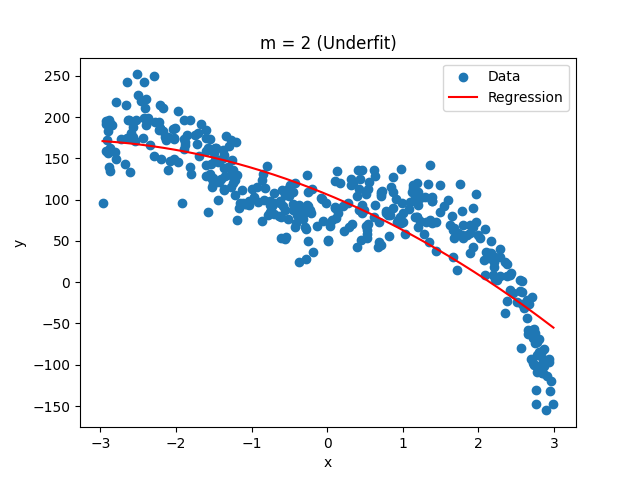
\includegraphics[width=0.9\textwidth]{../images/3/3_underfit.png}
		      \caption{Underfit model}
	      \end{figure}
	      \begin{figure}
		      \centering
		      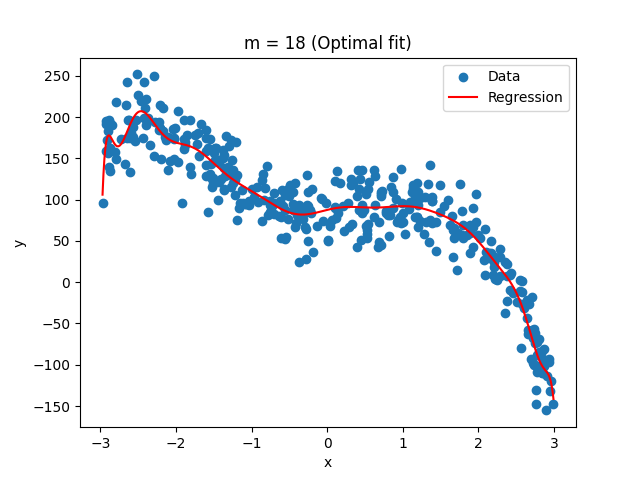
\includegraphics[width=0.9\textwidth]{../images/3/3_correctfit.png}
		      \caption{Optimal model}
	      \end{figure}
	      \begin{figure}
		      \centering
		      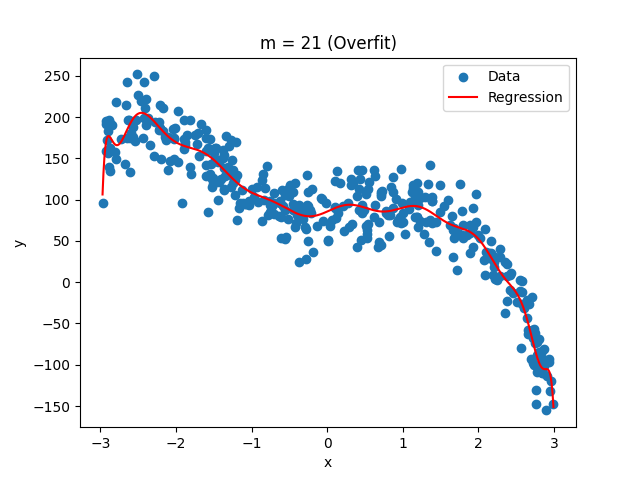
\includegraphics[width=0.8\textwidth]{../images/3/3_overfit.png}
		      \caption{Overfit model}
	      \end{figure}
	\item At the end these are the values obtained:
	      \begin{itemize}
		      \item $SS_R = 224592.60834798065$
		      \item $R^2 = 0.910251432520619$
	      \end{itemize}
\end{enumerate}
